\def \bottask {
	\item Докажите, что диагонали четырехугольника перпендикулярны $\iff$ суммы квадратов противолежащих сторон равны:
	  
	  \begin{minipage}[b]{0.6\textwidth}
	  $$AC^2 + BD^2 = BC^2 + AD^2 \iff \vec{AB}\ \bot\ \vec {CD}$$
	  \end{minipage}
	  %
	  \begin{minipage}{0.25\textwidth}
	  	\hspace*{1em}
	  	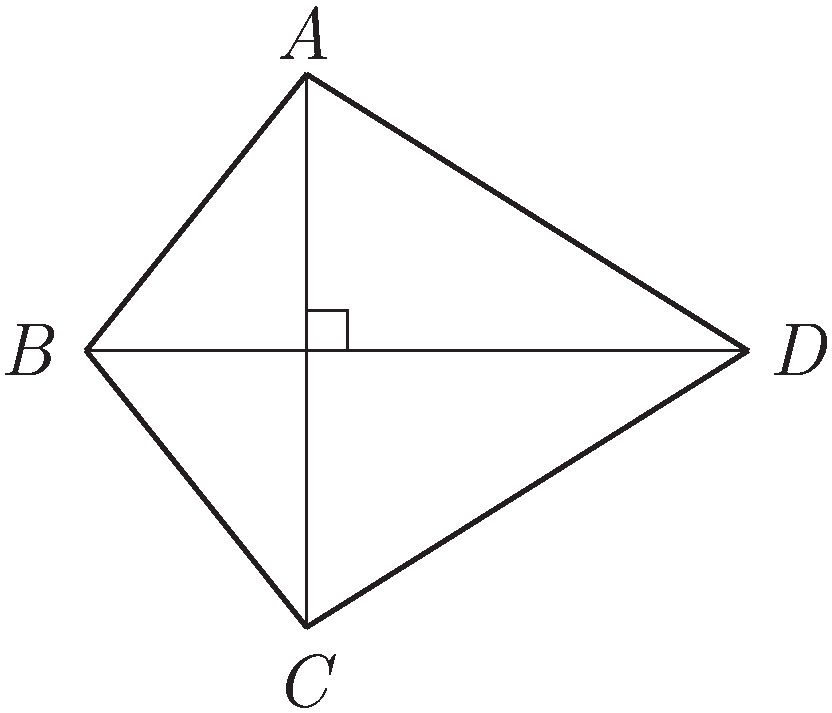
\includegraphics[width=\textwidth]{bot4}
	  \end{minipage}
}


\def \simple {
	\item Найти сумму ортогональных проекций вектора $\vec a$ на стороны правильного треугольника:
	\item В равнобедренном треугольнике медианы, проведённые к боковым сторонам, перпендикулярны. Найти все углы треугольника.
	\item Даны векторы $\vec a (\sqrt{3} \hspace{5} 3)^T$ и  $\vec b (1 \hspace{5} -1)^T$. Найти все вектора $\vec x$, образующие угол в $60^\cird$ с вектором $\vec a$ и $(\vec x, \vec b) = 1$.
	\item Объяснить при заданных $\vec a$ и $p$ геометрический смысл всех решений уравнения $(\vec x, \vec a) = p$
	\begin{tasks}(1)
		\task на плоскости
		\task в пространстве 
	\end{tasks}
	\item Доказать, что площадь произвольного выпуклого четырехугольника ABCD равна половине модуля векторного произведения $[\vec AC, \vec BD]$.
	\item Доказать, что для трёх неколлинеарных векторов $\vec a$, $\vec b$, $\vec c$ равенства $[\vec a, \vec b] = [\vec b, \vec c] = [\vec c, \vec a]$ выполняются тогда и только тогда, когда $\vec a + \vec b + \vec c = \vec 0$
	\item Стороны параллелограмма соотносятся как $m:n$, а угол между ними равен $\alpha$. Найти угол между диагоналями параллелограмма.
	
}

\def \easyA {
	\item Даны векторы $\vec a (\sqrt{3} \ 3)^T$ и  $\vec b (1\ -1)^T$. Найти все вектора $\vec x$, образующие угол в $60^\circ$ с вектором $\vec a$ и $(\vec x, \vec b) = 1$.
	
	\item Объяснить при заданных $\vec a$ и $p$ геометрический смысл всех решений уравнения $(\vec x, \vec a) = p$
	\begin{tasks}(1)
		\task на плоскости
		\task в пространстве 
	\end{tasks}
	
	\item В равнобедренном треугольнике медианы, проведённые к боковым сторонам, перпендикулярны. Найти все углы треугольника.
	
	
}

\def \easyB {
	\item Даны векторы $\vec a (\sqrt{3}\ 3)^T$ и
	$\vec b (1\  -1)^T$. Найти все векторы $\vec x$, образующие угол в $60^\circ$ с вектором $\vec a$ и $(\vec x, \vec b) = 1$.
	
	\item Объяснить при заданных $\vec a$ и $p$ геометрический смысл всех решений уравнения $(\vec x, \vec a) = p$
	\begin{tasks}(1)
		\task на плоскости
		\task в пространстве 
	\end{tasks}
	
	\item Стороны параллелограмма соотносятся как $m : n$, а угол между ними равен $\alpha$. Найти угол между диагоналями параллелограмма.
}

\def \easyC {
	\item Даны векторы $\vec a (\sqrt{3} \ 3)^T$
	и  $\vec b (1 \  -1)^T$. Найти все векторы $\vec x$, образующие угол в $60^\circ$ с вектором $\vec a$ и $(\vec x, \vec b) = 1$.
	
	\item Объяснить при заданных $\vec a$ и $\vec b$ геометрический смысл множества решений уравнения $[\vec x, \vec a] = \vec b$.
	
	\item Доказать, что площадь произвольного выпуклого четырехугольника ABCD равна половине модуля векторного произведения $[\vec{AC}, \vec{BD}]$.
	
}

\def \mediumA{
    	\item Объяснить при заданных $\vec a$ и $\vec b$ геометрический смысл множества решений уравнения $[\vec x, \vec a] = \vec b$.
	    
	    \item В равнобедренном треугольнике медианы, проведённые к боковым сторонам, перпендикулярны. Найти все углы треугольника.
	    
	    \item Доказать, что для трёх неколлинеарных векторов $\vec a$, $\vec b$, $\vec c$ равенства $[\vec a, \vec b] = [\vec b, \vec c] = [\vec c, \vec a]$ выполняются тогда и только тогда, когда $\vec a + \vec b + \vec c = \vec 0$
	
	
    	
}

\def \mediumB{
        \item Объяснить при заданных $\vec a$ и $\vec b$ геометрический смысл множества решений уравнения $[\vec x, \vec a] = \vec b$.
	    
	     \item В равнобедренном треугольнике медианы, проведённые к боковым сторонам, перпендикулярны. Найти все углы треугольника.
	     
	     \item Найти сумму ортогональных проекций вектора $\vec a$ на стороны правильного треугольника:
}

\def \mediumC{ 
        \item Объяснить при заданных $\vec a$ и $\vec b$ геометрический смысл множества решений уравнения $[\vec x, \vec a] = \vec b$.
	    
	    \item Стороны параллелограмма соотносятся как $m:n$, а угол между ними равен $\alpha$. Найти угол между диагоналями параллелограмма.
	    
	    
	    \item Доказать, что для трёх неколлинеарных векторов $\vec a$, $\vec b$, $\vec c$ равенства $[\vec a, \vec b] = [\vec b, \vec c] = [\vec c, \vec a]$ выполняются тогда и только тогда, когда $\vec a + \vec b + \vec c = \vec 0$

}

\def \mediumD{ 
        \item Объяснить при заданных $\vec a$ и $\vec b$ геометрический смысл множества решений уравнения $[\vec x, \vec a] = \vec b$.
	    
	   \item Стороны параллелограмма соотносятся как $m:n$, а угол между ними равен $\alpha$. Найти угол между диагоналями параллелограмма.
	    
	    
	    	\item Найти сумму ортогональных проекций вектора $\vec a$ на стороны правильного треугольника.

}

\def \mediumE{ 
        \item Объяснить при заданных $\vec a$ и $\vec b$ геометрический смысл множества решений уравнения $[\vec x, \vec a] = \vec b$.
	    
	    \item Доказать, что площадь произвольного выпуклого четырехугольника ABCD равна половине модуля векторного произведения $[\vec AC, \vec BD]$.
	    
	    
	    
	    
	    	\item Доказать, что для трёх неколлинеарных векторов $\vec a$, $\vec b$, $\vec c$ равенства $[\vec a, \vec b] = [\vec b, \vec c] = [\vec c, \vec a]$ выполняются тогда и только тогда, когда $\vec a + \vec b + \vec c = \vec 0$

}

\def \mediumF{ 
        \item Объяснить при заданных $\vec a$ и $\vec b$ геометрический смысл множества решений уравнения $[\vec x, \vec a] = \vec b$.
	    
	    \item Доказать, что площадь произвольного выпуклого четырехугольника ABCD равна половине модуля векторного произведения $[\vec {AC}, \vec {BD}]$.
	    
	    
	    
	    
	    	\item Найти сумму ортогональных проекций вектора $\vec a$ на стороны правильного треугольника.

}

\def \scalar_bred {
	\item Из одной точки отложены три вектора: $\vec a (0, -3, 4)^T$, $\vec b (4, 1, -8)^T$ и $\vec c$. Вектор~$\vec c$ имеет длину 1 и делит пополам угол между $\vec a$ и $\vec b$. Найдите координаты вектора~$\vec c$.
} 

\def \hardA {
		\item
			Объяснить при заданных $\vec a$ и $\vec b$ геометрический смысл множества решений уравнения $[\vec x, \vec a] = \vec b$.

    	\item В равнобедренном треугольнике медианы, проведённые к боковым сторонам, перпендикулярны. Найти все углы треугольника.
    	
    	\item Доказать, что для трёх неколлинеарных векторов $\vec a$, $\vec b$, $\vec c$ равенства $[\vec a, \vec b] = [\vec b, \vec c] = [\vec c, \vec a]$ выполняются тогда и только тогда, когда $\vec a + \vec b + \vec c = \vec 0$
    	
    	\item Найти сумму ортогональных проекций вектора $\vec a$ на стороны правильного треугольника.
	}
	
\def \hardB {

		\item Объяснить при заданных $\vec a$ и $\vec b$ геометрический смысл множества решений уравнения $[\vec x, \vec a] = \vec b$.

    	\item Стороны параллелограмма соотносятся как $m:n$, а угол между ними равен $\alpha$. Найти угол между диагоналями параллелограмма.
    	
    	\item Доказать, что для трёх неколлинеарных векторов $\vec a$, $\vec b$, $\vec c$ равенства $[\vec a, \vec b] = [\vec b, \vec c] = [\vec c, \vec a]$ выполняются тогда и только тогда, когда $\vec a + \vec b + \vec c = \vec 0$
    	
    	\item Найти сумму ортогональных проекций вектора $\vec a$ на стороны правильного треугольника.
	}
	
\def \hardC {
		\item Объяснить при заданных $\vec a$ и $\vec b$ геометрический смысл множества решений уравнения $[\vec x, \vec a] = \vec b$.

    	\item Доказать, что площадь произвольного выпуклого четырехугольника ABCD равна половине модуля векторного произведения $[\vec AC, \vec BD]$.
    	
    	\item Доказать, что для трёх неколлинеарных векторов $\vec a$, $\vec b$, $\vec c$ равенства $[\vec a, \vec b] = [\vec b, \vec c] = [\vec c, \vec a]$ выполняются тогда и только тогда, когда $\vec a + \vec b + \vec c = \vec 0$
    	
    	\item Найти сумму ортогональных проекций вектора $\vec a$ на стороны правильного треугольника.
	}
    	
    	
    	